
\chapter{Background and Related Work}
\label{ch:background}

This chapter provides background on the concepts related to predictive buffer management, and discusses other cache management approaches based on related ideas to those in this thesis.

\section{Optimal Cache Eviction}

Belady's MIN algorithm~\cite{beladyMIN} is known to be an optimal caching policy: for any sequence of accesses, it minimizes the number of accesses that are not satisfied by the cache and must access the next layer in the relevant storage hierarchy. It achieves this by evicting the cache item that will be accessed furthest in the future, which requires knowing future accesses. It is impossible to know future accesses in general so real-life systems are forced to use a (sub-optimal) heuristic policy, but MIN has inspired several more practical caching approaches. Predicting future accesses with a reasonable degree of accuracy enables better caching decisions by imitating MIN and evicting items not predicted to be accessed soon.


\section{Standard Database Buffer Cache Management}

Historically, databases used very simple heuristic strategies for buffer cache replacement such as \gls{lru}, \gls{lfu}, \gls{fifo}, clock~\cite{gclock}, \gls{lrd}, or some variant of one of these strategies.~\cite{effelsberg1984principles,hull1988buffer,feng1998study} Such strategies are still commonly used as they are simple to implement with low CPU overhead, and tend to be effective for common database access patterns.

Some more recent work on database cache management focuses on adapting the buffer cache to work well with other new technologies and advancements \cite{teng2017lsbm}, such as LSM-tree compaction leading to cache invalidation and extra avoidable storage access. Several works seek to adapt the existing heuristic approaches to perform better on flash drives, taking into account the distinct characteristics of solid-state storage and in particular the increased cost of writes compared to reads. \cite{ou2009cfdc,lv2011operation,jiang2015cost,hu2010pud,jin2012ad}


\section{Related Work Using Prediction}

Cache eviction is used in many contexts with different considerations, and as such there have been many cache eviction strategies that take inspiration from MIN, generally taking advantage of domain-specific details to create a practical caching strategy.

For CPU caches, Hawkeye~\cite{jain2016back} is a cache replacement strategy which simulates MIN on past accesses to identify which load instructions tend to be cache friendly or not. Several other works expand on this approach: Mockingjay~\cite{shah2022effective} uses a multi-class predictor instead of binary classification, and Harmony~\cite{jain2018rethinking} is based on a modified version of MIN that considers pre-fetching. Other strategies track or estimate time-to-reuse of cache lines to inform eviction strategies. \cite{keramidas2007cache, wu2011ship} % there are more of these...

In web content caching, \citet{famaey2013towards} predict future access distributions of web content to cache most frequently accessed items. \citet{yang2003web} build a model of user sessions to predict access probabilities of content based on the current sessions to inform caching decisions.


% ... os caching? ...

% \cite{yoon2002buffer} -- detect access patterns

% ... db caching ...

For database caching, \citet{yuan2022learned} propose two machine-learning based buffer cache eviction strategies trained on historical accesses: one which classifies buffers as cache friendly or cache averse similar to Hawkeye, and the other which predicts time-of-next-access to mimic MIN more directly.
%\footnote{...: the paper is focused on the machine learning aspect, and they do not seem to discuss how they actually select the buffer based on these stats beyond ``pick the largest one''. I think they only tested in a simulator without measuring CPU overhead.}
%\footnote{...: this and PBM are the only database-specific predictive approaches I found}
Instead of \textit{predicting} future accesses, \cite{coopScans} instead reorders future accesses for long-running scans to improve the cache usage.

Prior work that takes inspiration from MIN most related to this thesis are \cite{relaxedBelady} and \cite{pbm}. 

\citet{relaxedBelady} use machine learning to estimate access times and a similar technique to the one described in Chapter~\ref{sec:PBM-sampling} to choose what to evict, but applied to content distribution networks instead of database buffer caching. Some key differences between content distribution and database buffer management motivate a slightly different approach: content distribution caches can afford a higher CPU cost since the cache items are much larger and the latency penalty of a cache miss is higher, and databases have more information available about near-future accesses.

\citet{pbm} focus on database caching under a workload with mostly sequential access, and leverage knowledge about the currently active queries to estimate the future access pattern. The approach presented in this thesis has some overlap with this approach, so the techniques from \cite{pbm} are summarized in Chapter~\ref{sec:pbm-pq_summary}.

\section{Summary of Priority-Queue Based Predictive Buffer Management}
\label{sec:pbm-pq_summary}

Prior approach \cite{pbm} tracks information about active sequential scans in the database to predict when different parts of the data will be accessed next. \textcolor{blue}{\Cref{fig:scan_tracking} shows an example of how my implementation in PostgreSQL tracks this information.} When a scan starts, based on the information in the query, the scan registers itself indicating the set of blocks it will eventually access and when it will access those blocks. For each block, the system stores a list of the scans that will access that block. When a scan reaches a particular block it removes itself from that block's list of scans since the same sequential scan will not return to the same block.

As the scan progresses, it tracks its current position and speed, which together are used to estimate when it will reach a particular data block assuming it will maintain the current scan speed.

As mentioned previously, making the actual decisions about what to evict must be done quickly. In the approach from \cite{pbm} that will be referred to as PBM-PQ in this thesis, the authors found that storing the buffers in a true priority queue was too slow and instead developed an approximate priority queue with $O(1)$ insertion and removal to alleviate this concern. The approximate priority queue, depicted in Figure \ref{fig:approx-pq}, groups database blocks into a fixed number of buckets based on the estimated time to next access, with buckets further in the future having exponentially wider ranges than buckets to be accessed sooner.

Cached blocks are inserted into the approximate priority queue or moved between buckets in the queue when it is loaded into the cache or when the set of scans that will access it changes, i.e., when a new scan starts or an existing scan has finished processing that block. As time progresses, the priority -- corresponding to the time to next access -- of each block decreases, so the buckets are periodically shifted to correspond to earlier time intervals with the earliest bucket being removed. Eviction candidates are chosen from the non-empty bucket furthest in the future, which should have the next-access furthest in the future to mimic MIN.

\begin{figure}
    \centering
    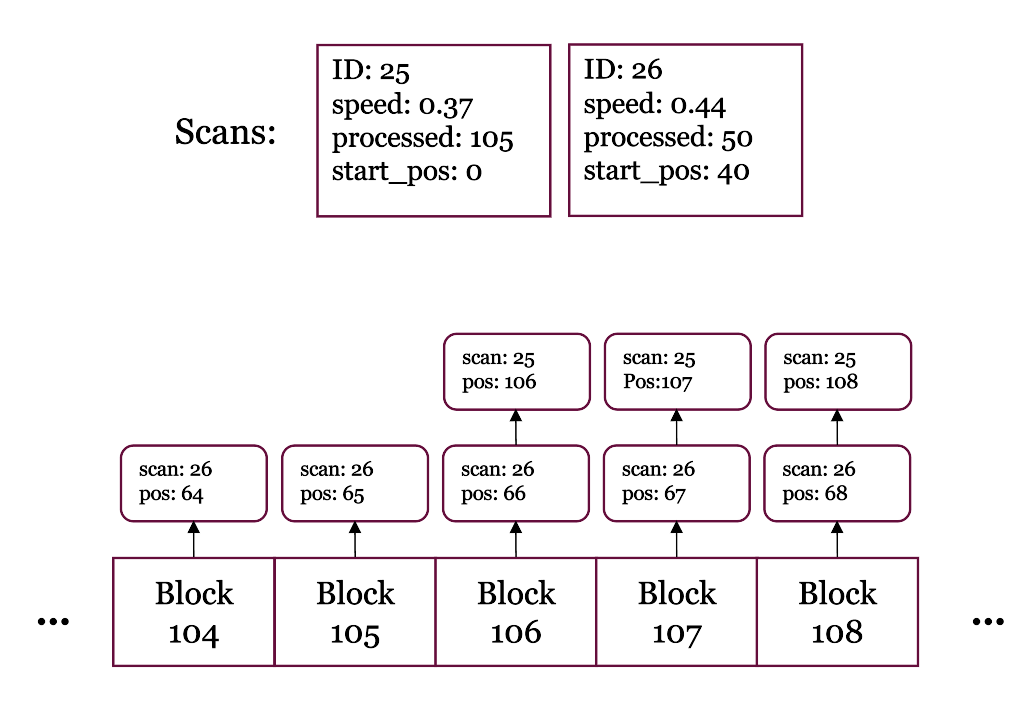
\includegraphics[width=1\columnwidth]{figures/Diagrams/seq_scan_registered_progress.png}
    \caption[PBM sequential scan tracking]{\textcolor{blue}{How PBM tracks sequential scans. A list of relevant scans is tracked for each block in the database. When a scan starts, it adds itself to the list for each relevant block, and removes itself after the scan has passed that block. Time of access for each scan is estimated based on the scan speed and the distance from the scan to the block, based on block position and current scan position. Then the estimated next-access-time of the block is the minimum access time over the list of scans.}}
    \label{fig:scan_tracking}
\end{figure}

\begin{figure}
    \centering
    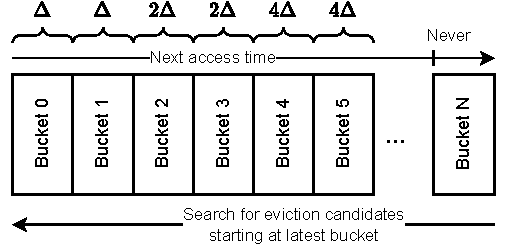
\includegraphics[width=1\columnwidth]{figures/Diagrams/diagrams-approx-PQ.pdf}
    \caption[PBM-PQ's approximate priority queue]{Structure of the approximate priority queue used by PBM-PQ. The time range associated with each bucket increases exponentially for later buckets, and $\Delta$ is the time range of the first buckets.}
    \label{fig:approx-pq}
\end{figure}